\documentclass[aspectratio=169,xcolor=table]{beamer}
\usepackage[utf8]{inputenc}
\usepackage[T1,T5]{fontenc}
\usepackage{amsmath,amssymb,booktabs,array,graphicx,tikz}
\usetikzlibrary{positioning,arrows.meta,fit,calc}

\definecolor{Primary}{HTML}{111B88}
\definecolor{Secondary}{HTML}{101659}
\definecolor{Accent}{HTML}{F2A900}
\definecolor{SoftBlue}{HTML}{EAF2F8}
\definecolor{TextGray}{HTML}{4D5966}
\definecolor{RiskRed}{HTML}{A23B3B}
\definecolor{GoodGreen}{HTML}{26734D}
\mode<presentation>{\usetheme{Madrid}\usecolortheme{default}\setbeamertemplate{navigation symbols}{}}
\setbeamercolor{structure}{fg=Primary}
\setbeamercolor{frametitle}{fg=white,bg=Primary}
\setbeamercolor{title}{fg=white,bg=Primary}
\setbeamercolor{block body}{fg=black,bg=SoftBlue}
\setbeamercolor{block body alerted}{fg=black,bg=Accent!12}
\setbeamercolor{section in head/foot}{fg=white,bg=Primary}
\setbeamercolor{author in head/foot}{fg=white,bg=Secondary}
\setbeamercolor{date in head/foot}{fg=white,bg=Primary}
\setbeamerfont{section in head/foot}{size=\tiny,series=\bfseries}
\setbeamerfont{author in head/foot}{size=\scriptsize}
\setbeamerfont{date in head/foot}{size=\scriptsize,series=\bfseries}
\setbeamerfont{frametitle}{series=\bfseries}
\setbeamerfont{title}{series=\bfseries}
\newcommand{\decklabel}{Contextual ASR -- Scorer}
\setbeamertemplate{itemize item}{\color{Secondary}$\blacktriangleright$}
\setbeamertemplate{itemize subitem}{\color{Accent}$\bullet$}
\setbeamertemplate{headline}{\leavevmode\begin{beamercolorbox}[wd=\paperwidth,ht=2.7ex,dp=1.1ex,leftskip=.35cm,rightskip=.35cm]{section in head/foot}\insertsectionnavigationhorizontal{\dimexpr\paperwidth-.70cm\relax}{}{}\end{beamercolorbox}}
\setbeamertemplate{footline}{\leavevmode\hbox{\begin{beamercolorbox}[wd=.55\paperwidth,ht=2.6ex,dp=1ex,leftskip=.35cm,rightskip=.20cm]{section in head/foot}\usebeamerfont{section in head/foot}\insertsectionhead\end{beamercolorbox}\begin{beamercolorbox}[wd=.27\paperwidth,ht=2.6ex,dp=1ex,center]{author in head/foot}\usebeamerfont{author in head/foot}\decklabel\end{beamercolorbox}\begin{beamercolorbox}[wd=.18\paperwidth,ht=2.6ex,dp=1ex,rightskip=.35cm plus1fil]{date in head/foot}\usebeamerfont{date in head/foot}\hfill\insertframenumber\,/\,\inserttotalframenumber\end{beamercolorbox}}}
\newcolumntype{L}[1]{>{\raggedright\arraybackslash}p{#1}}
\newcommand{\hi}[1]{\textcolor{Primary}{\textbf{#1}}}
\newcommand{\bad}[1]{\textcolor{RiskRed}{\textbf{#1}}}
\newcommand{\good}[1]{\textcolor{GoodGreen}{\textbf{#1}}}
\newcommand{\src}[1]{{\tiny\color{TextGray}[#1]}}
\newcommand{\ra}{$\rightarrow$}
\newcommand{\nbox}[2][block body]{\begin{beamercolorbox}[sep=0.45em,rounded=true]{#1}\footnotesize #2\end{beamercolorbox}}
\newcommand{\bignum}[3]{\begin{beamercolorbox}[sep=0.5em,rounded=true,center]{block body}{\Large\hi{#1}}\par\vspace{0.05cm}{\scriptsize #2}\par{\tiny\color{TextGray}#3}\end{beamercolorbox}}

\title{Scorer biết từ nằm ở đâu}
\subtitle{Chọn từ tốt hơn và đẩy từ vào ASR đúng lúc, không cần prompt}
\author{Nhóm Contextual ASR}
\institute{}
\date{20/11/2026}
\setbeamertemplate{title page}{\begin{centering}\vspace*{0.10cm}
\includegraphics[height=1.08cm]{../2026-10-23/imgs/logo.png}\par\vspace{0.32cm}\begin{beamercolorbox}[sep=0.50em,center,rounded=true]{title}\usebeamerfont{title}\inserttitle\par\vspace{0.14cm}{\small\insertsubtitle\par}\end{beamercolorbox}\vspace{0.42cm}{\usebeamerfont{author}\insertauthor\par}\vspace{0.10cm}{\usebeamerfont{institute}\insertinstitute\par}\vfill{\usebeamerfont{date}\insertdate\par}\end{centering}}

\begin{document}
\begin{frame}[plain]\titlepage\end{frame}

% ==================================================================
\section{Tóm tắt}
\begin{frame}{Buổi này: một ý chính, ba con số}
\nbox[block body alerted]{\textbf{Ý chính.} Scorer biết \hi{từ nằm ở giây nào} thì (1) chọn từ đúng tốt hơn hẳn, và (2) cho phép \hi{đẩy từ vào ASR đúng lúc} mà không cần prompt. Trên IS21 LibriSpeech, cách này \good{thắng Hou25 về B-WER}, có ý nghĩa thống kê.}
\vspace{0.25cm}
\begin{columns}[T]
\column{0.32\textwidth}\bignum{73 \ra{} 89}{Sạch@1: từ đúng đứng đầu list}{test-other, list 2000 từ; Hou25 \ra{} scorer mới}
\column{0.32\textwidth}\bignum{9.69 \ra{} 7.53}{B-WER khi đưa vào Whisper}{Hou25 prompt \ra{} đẩy có vị trí; $\Delta$ = $-$2.16 [$-$2.89; $-$1.54]}
\column{0.32\textwidth}\bignum{0 prompt}{không phụ thuộc cách viết prompt}{chỉ cần logits + tokenizer của ASR}
\end{columns}
\vspace{0.25cm}
{\footnotesize Chạy 14--15/11 trên 2$\times$RTX 4090. Mọi scorer train trên train-clean-100. ASR: Whisper-large-v3-turbo đóng băng. \textbf{Hou25 ở đây là bản tái hiện của nhóm} (2 epoch). Số liệu: \texttt{scorer/analysis/REPORT-1115.md}.}
\end{frame}

% ==================================================================
\section{Bài toán}
\begin{frame}{Bài toán và mốc so sánh: Hou25 bỏ mất thông tin vị trí}
\centering
\begin{tikzpicture}[font=\footnotesize,>={Stealth},
  box/.style={draw=Primary,fill=SoftBlue,rounded corners=2pt,minimum height=0.9cm,align=center,inner sep=4pt},
  bad/.style={draw=RiskRed,fill=RiskRed!10,rounded corners=2pt,minimum height=0.9cm,align=center,inner sep=4pt,thick}]
\node[box] (a) at (0,0) {audio};
\node[box] (l) at (0,-1.6) {list\\2000 từ};
\node[box] (tts) at (2.5,-1.6) {TTS từng từ};
\node[box] (m) at (5.2,-0.8) {bản đồ giống nhau\\\scriptsize từ $\times$ thời gian};
\node[bad] (p) at (8.2,-0.8) {CNN +\\\textbf{lấy trung bình}\\\textbf{cả bản đồ}};
\node[box] (k) at (10.9,-0.8) {top-50\\\scriptsize (cả câu)};
\node[bad] (w) at (13.4,-0.8) {\textbf{prompt}\\Whisper};
\draw[->,thick] (a) -- (m); \draw[->,thick] (l) -- (tts); \draw[->,thick] (tts) -- (m);
\draw[->,thick] (m) -- (p); \draw[->,thick] (p) -- (k); \draw[->,thick] (k) -- (w);
\node[font=\scriptsize,text=RiskRed,align=center] at (8.2,-2.2) {vị trí của từ\\bị vứt ở đây};
\node[font=\scriptsize,text=RiskRed,align=center] at (13.4,-2.2) {phụ thuộc thứ tự,\\độ dài, cách viết prompt};
\end{tikzpicture}
\vspace{0.35cm}
\begin{columns}[T]
\column{0.49\textwidth}
\nbox{\textbf{Hou25} (Interspeech 2025): scorer TTS + CNN, top-50 đưa vào prompt. Mốc so trực tiếp: IS21, LibriSpeech test-clean / test-other, N100--2000, B-WER.}
\column{0.49\textwidth}
\nbox{\textbf{Câu hỏi buổi này:} giữ lại vị trí thì (1) scorer chọn từ tốt hơn không, và (2) ASR có dùng được vị trí để viết đúng hơn mà không cần prompt không?}
\end{columns}
\end{frame}

\begin{frame}{Đo lại cho công bằng: ``lọt top-50'' che mất khác biệt}
\begin{columns}[T]
\column{0.60\textwidth}
\centering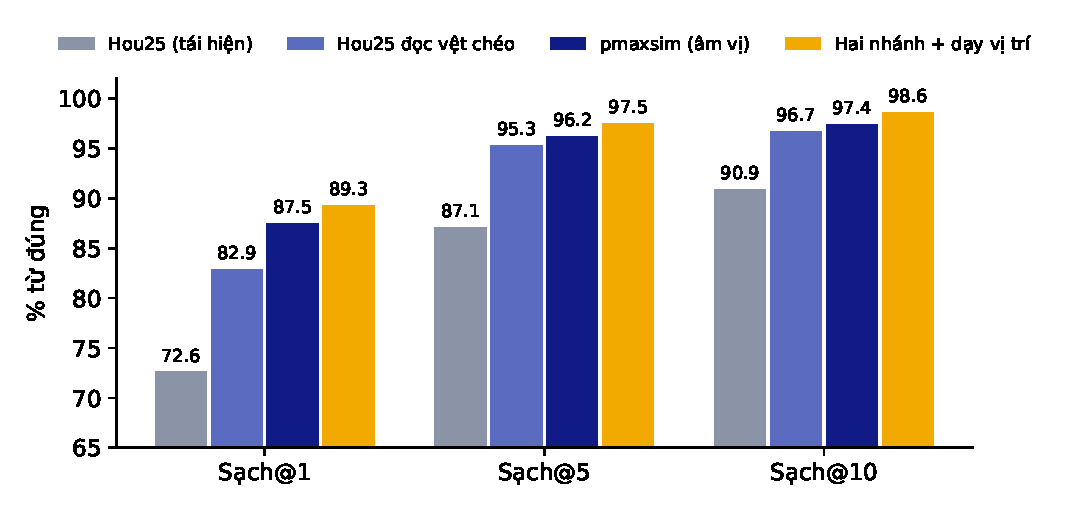
\includegraphics[width=\linewidth]{imgs/sach_k.pdf}
\column{0.39\textwidth}
\nbox{\textbf{Sạch@K:} \% từ đúng có ít hơn K từ nhiễu đứng trên nó.}
\vspace{0.12cm}
\nbox{Ở mốc 50 (Hou25 báo): 95.4 so với 98.4, cách 3 điểm. Ở mốc 1: 72.6 so với 87.5, \bad{cách 15 điểm}.}
\vspace{0.12cm}
\nbox{Top-50 của Hou25: mỗi câu 1--2 từ đúng đi kèm $\sim$48 từ nhiễu, \bad{precision 3--4\%}. Khi bỏ prompt, mỗi từ nhiễu bị đẩy vào là một lỗi chèn.}
\end{columns}
\src{test-other, list N2000; REPORT-1115 mục 2, 3, 5, 7c}
\end{frame}

\begin{frame}{Hou25 sai vì đâu: báo nhầm từ khác hẳn, tăng theo độ dài câu}
\begin{columns}[T]
\column{0.56\textwidth}
\centering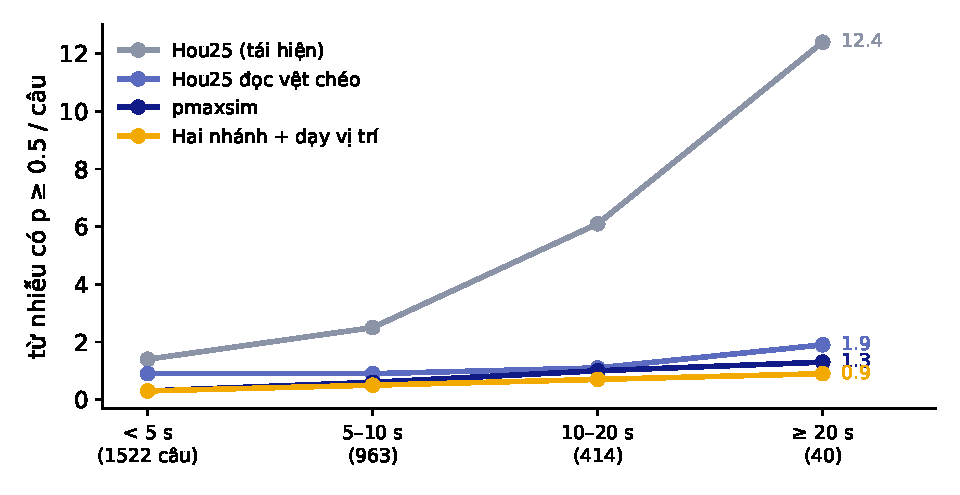
\includegraphics[width=\linewidth]{imgs/bao_nham.pdf}
\column{0.43\textwidth}
\nbox{Khi từ đúng bị vượt, từ vượt lên là \bad{từ khác hẳn} trong 96\% số lượt; từ gần âm chỉ 3\%.}
\vspace{0.12cm}
\nbox{76\% từ báo nhầm của Hou25 \bad{không giống đoạn âm nào} trong câu (scorer âm vị: 40\%).}
\vspace{0.12cm}
\nbox{Câu càng dài, Hou25 càng báo nhầm: 1.4 \ra{} 12.4 từ/câu. Scorer âm vị gần như phẳng.}
\vspace{0.12cm}
{\footnotesize \textbf{Diễn giải:} lấy trung bình cả bản đồ thì câu dài có nhiều mảng ngẫu nhiên ``giống vệt'' \ra{} từ nhiễu bị đẩy lên.}
\end{columns}
\src{test-other N2000; REPORT-1115 mục 3; SMALL\_R N2--N4}
\end{frame}

% ==================================================================
\section{Kết quả scorer}
\begin{frame}{Kết quả 1: giả thuyết của Hoàng đúng khi train lại}
\begin{columns}[T]
\column{0.58\textwidth}
\renewcommand{\arraystretch}{1.15}\footnotesize
\begin{tabular}{L{2.6cm}cccc}
\toprule
Hou25, cách gộp & Sạch@1 & báo nhầm & từ ASR & định vị \\
 & & câu $\geq$20 s & nghe sai & trúng \\
\midrule
trung bình (gốc) & 73.3 & 6.1 & 46.3 & 79\% \\
top-k frame & 73.8 & 8.0 & 47.2 & 4\% \\
\rowcolor{Accent!15}\textbf{vệt chéo} & \textbf{82.9} & \textbf{1.9} & \textbf{60.9} & \textbf{99\%} \\
\bottomrule
\end{tabular}
\vspace{0.2cm}

{\footnotesize Cùng dữ liệu, seed, số epoch; chỉ khác bước gộp. $\Delta$Sạch@1 = \good{+9.5 [+7.9; +11.2]}.}
\column{0.40\textwidth}
\nbox{\textbf{Giả thuyết (Hoàng, F14):} bản đồ S1 của Hou25 có vệt chéo đúng chỗ từ được nói; lấy trung bình làm mất nó.}
\vspace{0.12cm}
\nbox{Trước đây chỉ đổi cách gộp lúc test \ra{} không lợi (A1). \good{Train lại thì lợi rõ}, và cùng một model định vị được từ.}
\vspace{0.12cm}
\nbox[block body alerted]{Top-k không giúp \ra{} thứ có ích là \hi{hình dạng vệt} (đúng thứ tự, liền nhau), không phải ``đọc cục bộ'' nói chung.}
\end{columns}
\src{test-other N2000, 2939 câu; REPORT-1115 mục 5}
\end{frame}

\begin{frame}{Kết quả 2: scorer hai nhánh có dạy vị trí}
\begin{columns}[T]
\column{0.50\textwidth}
\centering
\begin{tikzpicture}[font=\tiny,>={Stealth},
  box/.style={draw=Primary,fill=SoftBlue,rounded corners=2pt,minimum height=0.6cm,align=center,inner sep=2pt},
  acc/.style={draw=Accent,fill=Accent!15,rounded corners=2pt,minimum height=0.6cm,align=center,inner sep=2pt,thick}]
\node[box,text width=1.55cm] (a) at (0,0) {audio \ra{} encoder Whisper (đóng băng)};
\node[box,text width=1.55cm] (w) at (0,-1.5) {từ \ra{} âm vị (g2p, không TTS)};
\node[box,text width=1.35cm] (m1) at (2.25,0) {bản đồ 1\\âm vị $\times$ frame};
\node[box,text width=1.35cm] (m2) at (2.25,-1.5) {bản đồ 2\\âm vị $\times$ frame};
\node[acc,text width=2.15cm] (b1) at (4.6,0) {\textbf{khớp tự do}: mỗi âm vị tìm frame giống nhất \ra{} \good{ít sót}};
\node[acc,text width=2.15cm] (b2) at (4.6,-1.5) {\textbf{khớp đúng thứ tự}: đường đi đơn điệu \ra{} \good{loại nhiễu, ra biên}};
\node[box] (o) at (4.6,-2.85) {(từ, $p$, $t_{\text{đầu}}$, $t_{\text{cuối}}$)};
\draw[->] (a.east) -- (m1.west); \draw[->] (a.east) -- (m2.west);
\draw[->] (w.east) -- (m1.west); \draw[->] (w.east) -- (m2.west);
\draw[->] (m1) -- (b1); \draw[->] (m2) -- (b2);
\draw[->] (b1.east) -- ++(0.2,0) |- (o.east); \draw[->] (b2.south) -- (o.north);
\node[text=TextGray,align=center] at (1.1,-2.85) {train: từ đúng chỉ được tính\\điểm trong đoạn MFA của nó\\(\textbf{dạy vị trí})};
\end{tikzpicture}
\column{0.48\textwidth}
\renewcommand{\arraystretch}{1.1}\scriptsize
\begin{tabular}{L{2.65cm}ccc}
\toprule
test-other N2000 & Sạch@1 & nghe giống & ASR sai \\
\midrule
Hou25 (tái hiện) & 72.6 & 51.4 & 45.9 \\
pmaxsim (khớp tự do) & 87.5 & 64.7 & 64.5 \\
\quad + dạy vị trí & 88.3 & 65.0 & 65.9 \\
khớp đúng thứ tự + dạy vị trí & 88.3 & 65.3 & 69.2 \\
\rowcolor{Accent!15}\textbf{hai nhánh, 1 model} & \textbf{89.3} & \textbf{67.7} & \textbf{70.9} \\
cộng điểm 2 model riêng & 90.8 & 69.6 & -- \\
\bottomrule
\end{tabular}
\vspace{0.1cm}

{\scriptsize Định vị: sai số tâm \good{0.02 s}, 99\% trúng đoạn. test-clean: 93.4 \ra{} 94.7. Hai nhánh cần \textbf{bản đồ riêng}; dùng chung chỉ được 88.3. Chấm 4--7 ms/câu, nhanh hơn Hou25 $\sim$200 lần.}
\end{columns}
\src{REPORT-1115 mục 3, 6, 6c, 7c; ``nghe giống'' = list hard\_N2000; ``ASR sai'' = từ Whisper không prompt nghe sai}
\end{frame}

\begin{frame}{Kết quả 3: có vị trí thì lọc được list}
\begin{columns}[T]
\column{0.64\textwidth}
\centering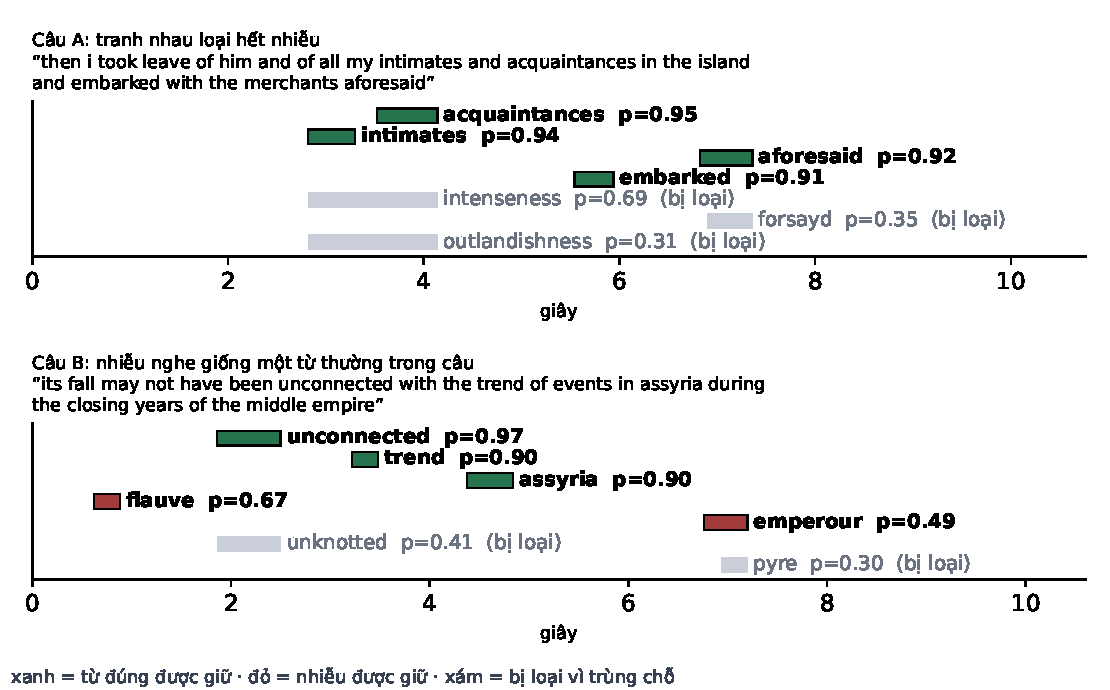
\includegraphics[width=\linewidth]{imgs/tranh_nhau.pdf}
\column{0.35\textwidth}
\nbox{\textbf{Luật:} hai từ không thể ở cùng một chỗ \ra{} từ có đoạn trùng với từ điểm cao hơn bị loại.}
\vspace{0.12cm}
\nbox{2000 từ \ra{} \hi{$\sim$2 từ/câu}, \good{precision 91\%}, vẫn giữ 91\% từ đúng (top-50 Hou25: precision 3--4\%).}
\vspace{0.12cm}
\nbox[block body alerted]{Câu B: ``flauve'' nghe như ``fall'', ``emperour'' như ``empire''. Từ nhiễu khớp một \bad{từ thường} trong câu \ra{} chưa xử lý được.}
\end{columns}
\src{test-other; hai câu thật, scorer hai nhánh 1 model, p $\geq$ 0.3; precision ở dòng giữa: bản cộng điểm, p $\geq$ 0.5 (REPORT-1115 mục 4, 6c)}
\end{frame}

% ==================================================================
\section{Đưa vào ASR}
\begin{frame}{Kết quả 4: đẩy từ đúng lúc vào Whisper, không cần prompt}
\begin{columns}[T]
\column{0.62\textwidth}
\renewcommand{\arraystretch}{1.12}\footnotesize
\begin{tabular}{L{4.0cm}cc}
\toprule
WER / B-WER & test-other & test-clean \\
\midrule
không context & 4.25 / 17.92 & 2.16 / 8.64 \\
\textbf{Hou25}: prompt top-50 & 3.39 / 9.69 & 1.66 / 5.15 \\
scorer mới: prompt top-50 & 3.43 / 10.03 & -- \\
scorer mới: đẩy \textbf{không} vị trí & 3.56 / 7.17 & -- \\
\rowcolor{Accent!15}\textbf{scorer mới: đẩy có vị trí} & \textbf{3.14} / \textbf{7.53} & \textbf{1.59} / \textbf{3.93} \\
scorer mới: prompt + đẩy có vị trí & 3.22 / \textbf{6.76} & \textbf{1.47} / \textbf{3.12} \\
\midrule
trần: đúng từ + vị trí MFA & 2.99 / 5.99 & 1.53 / 2.77 \\
\bottomrule
\end{tabular}
\column{0.36\textwidth}
\nbox{\textbf{Cách đẩy:} khi decoder đang nghe trong đoạn của từ, cộng $\lambda$ vào log-prob token của từ; mỗi từ đẩy một lần.}
\vspace{0.1cm}
\nbox{So với Hou25, B-WER:\\
other \good{$-$2.16 [$-$2.89; $-$1.54]}\\
clean \good{$-$1.22 [$-$1.76; $-$0.68]}\\
U-WER không đổi.}
\vspace{0.1cm}
\nbox[block body alerted]{WER tổng $-$0.25 [$-$0.47; +0.03]: \bad{chưa có ý nghĩa}. Thêm prompt thì có ý nghĩa.}
\end{columns}
\src{N2000; scorer mới = cộng điểm hai nhánh có dạy vị trí; bản 1 model: 3.22 / 7.65 và 1.58 / 3.83; tham số chọn trên dev-other (REPORT-1115 mục 7b, 7c)}
\end{frame}

\begin{frame}{Ba phát hiện về phía ASR}
\begin{columns}[T]
\column{0.32\textwidth}
\nbox[block body alerted]{\textbf{\textcircled{\scriptsize 1} Kênh prompt đã bão hoà.}\\[2pt]
Scorer tốt hơn 17 điểm Sạch@1, mà đưa top-50 vào prompt: B-WER 10.03, \bad{không hơn} Hou25 (9.69).\\[2pt]
\ra{} Lợi ích của scorer tốt chỉ lấy được qua \hi{vị trí + đẩy logit}.}
\column{0.32\textwidth}
\nbox{\textbf{\textcircled{\scriptsize 2} Whisper cần vị trí.}\\[2pt]
Cùng list $\sim$2 từ/câu:\\
đẩy mọi lúc: WER 3.56\\
đẩy đúng lúc: WER \good{3.14}\\
$\Delta$ = $-$0.42 [$-$0.51; $-$0.34]\\[2pt]
Đẩy mọi lúc làm \bad{U-WER tăng} (2.62 \ra{} 3.13): từ bị viết đè lên từ thường.}
\column{0.32\textwidth}
\nbox{\textbf{\textcircled{\scriptsize 3} Còn 1.5 điểm B-WER tới trần.}\\[2pt]
Trần (đúng từ, đúng chỗ): 5.99.\\
Hiện tại: 7.53.\\[2pt]
Trên dev: khoảng một nửa do \textbf{vị trí} chưa chuẩn, một nửa do \textbf{list} chưa chuẩn (sót từ + nhiễu).}
\end{columns}
\vspace{0.3cm}
\nbox[block body alerted]{\textbf{Hệ quả cho hướng đi:} đầu tư vào scorer chỉ có lời khi đầu ra của nó là \hi{(từ, $p$, vị trí)} và được dùng \hi{lúc decode}; cải thiện thứ hạng top-50 rồi đưa vào prompt thì không.}
\src{test-other N2000 (REPORT-1115 mục 7b)}
\end{frame}

% ==================================================================
\section{Còn thiếu và kế hoạch}
\begin{frame}{Còn thiếu}
\renewcommand{\arraystretch}{1.25}\footnotesize
\begin{tabular}{L{4.4cm}L{5.0cm}L{4.4cm}}
\toprule
Vấn đề & Số đo & Hướng xử lý \\
\midrule
WER tổng chưa thắng Hou25 có ý nghĩa & $-$0.25 [$-$0.47; +0.03] (không prompt) & giảm nhiễu bị đẩy vào; scorer cuối train 960h \\
Audio không có từ nào trong list & WER 4.49 so với 4.25 (không context) & train khối ``tranh nhau + \textbf{không từ nào}'' thay luật bằng tay \\
Một model kém bản cộng điểm & 89.3 so với 90.8 Sạch@1; điểm dev dao động 84.8--90.2 giữa các epoch & loss riêng cho từng nhánh; lấy trung bình ckpt; dev lớn hơn \\
Nhiễu khớp một từ thường trong câu & ``flauve'' $\sim$ ``fall'', ``emperour'' $\sim$ ``empire'' & dùng bản chép lần 1 của ASR làm bằng chứng phủ định \\
Phạm vi so sánh & Hou25 là bản tái hiện; chỉ Whisper & ckpt của Hoàng; Hou25-vệt-chéo làm baseline mạnh; Qwen3-ASR \\
\bottomrule
\end{tabular}
\vspace{0.2cm}

{\footnotesize Đã thử và bỏ: train với 16 từ nhiễu/từ đúng (kém hơn 4); top-k thay cho vệt chéo; lọc thêm theo top-k của ASR.}
\end{frame}

\begin{frame}{Kế hoạch đến hạn Interspeech (09/02/2027) và xin ý kiến thầy}
\centering
\begin{tikzpicture}[font=\scriptsize,>={Stealth}]
\draw[->,thick,Primary] (0,0) -- (14.2,0);
\foreach \xx/\dd/\tt in {0.6/20.11/họp hôm nay, 4.0/20.12/scorer cuối, 8.0/17.01/đủ bảng, 11.6/05.02/bản nộp}{
  \fill[Accent] (\xx,0) circle (3pt);
  \node[above,font=\scriptsize\bfseries] at (\xx,0.12) {\dd};
  \node[below,font=\scriptsize] at (\xx,-0.12) {\tt};}
\end{tikzpicture}
\vspace{0.15cm}
\begin{columns}[T]
\column{0.49\textwidth}
\nbox{\textbf{Đến 20/12 -- scorer cuối:} một model hai nhánh $\geq$ 90.5 Sạch@1; khối ``không từ nào'' được train; train 960h (trước đây +1.8 Sạch@1).\\[2pt]
\textbf{Đến 17/01 -- đủ bảng:} N100--2000 $\times$ 2 tập; ckpt Hou25 của Hoàng; Hou25-vệt-chéo; Qwen3-ASR.\\[2pt]
\textbf{Đến 05/02 -- viết bài:} 4 trang, 3--4 bảng.}
\column{0.49\textwidth}
\nbox[block body alerted]{\textbf{Xin ý kiến thầy:}\\[2pt]
\textcircled{\scriptsize 1} Đóng góp chính đặt ở \textbf{scorer hai nhánh có vị trí}, ở \textbf{đẩy logit theo vị trí, không cần prompt}, hay gộp cả hai thành một hệ?\\[2pt]
\textcircled{\scriptsize 2} Mốc so: chỉ Hou25, hay thêm PTC-Bias và boost không gate (Liu 2508.17796)?\\[2pt]
\textcircled{\scriptsize 3} Whisper + Qwen3-ASR đã đủ, hay cần thêm một SpeechLLM?}
\end{columns}
\end{frame}

% ==================================================================
\section{Dự phòng}
\begin{frame}{Dự phòng 1: thước đo}
\renewcommand{\arraystretch}{1.25}\footnotesize
\begin{tabular}{L{3.0cm}L{10.6cm}}
\toprule
Thước đo & Nghĩa \\
\midrule
Sạch@K & \% từ đúng có ít hơn K từ \textbf{nhiễu} đứng trên nó (không tính từ đúng khác, để câu nhiều từ hiếm không bị phạt oan) \\
Đúng@chỗ & tại đoạn audio của từ đúng (MFA), nó có đứng trên mọi từ nhiễu được scorer đặt cùng chỗ không \\
Định vị & sai số tâm (giây) và \% tâm nằm trong đoạn thật $\pm$ 0.1 s \\
Báo nhầm & số từ nhiễu có $p \geq 0.5$ mỗi câu, chia theo độ dài câu \\
WER / U-WER / B-WER & scorer IS21 chính thức (thay = 4, chèn/xoá = 3), chuẩn hoá Whisper; B-WER tính trên từ hiếm của reference \\
CI 95\% & bootstrap ghép cặp theo câu, 1000 lần \\
\bottomrule
\end{tabular}
\end{frame}

\begin{frame}{Dự phòng 2: list nhiều từ nghe giống, và theo cỡ list}
\begin{columns}[T]
\column{0.48\textwidth}
\renewcommand{\arraystretch}{1.12}\footnotesize
\begin{tabular}{L{3.2cm}cc}
\toprule
hard\_N2000, test-other & Sạch@1 & $\Delta$ \\
\midrule
Hou25 (TTS) & 51.4 & \\
pmaxsim (âm vị) & 64.7 & \\
khớp đúng thứ tự & 60.5 & \\
\rowcolor{Accent!15}hai nhánh, 1 model & 67.7 & +3.0 \\
cộng điểm 2 model & 69.6 & +4.6 \\
\bottomrule
\end{tabular}
\vspace{0.15cm}

{\footnotesize TTS \bad{không} cho lợi thế với từ nghe giống. Trên list này 21\% số lần từ đúng bị vượt là do từ gần âm (list thường: 3--7\%).}
\column{0.50\textwidth}
\centering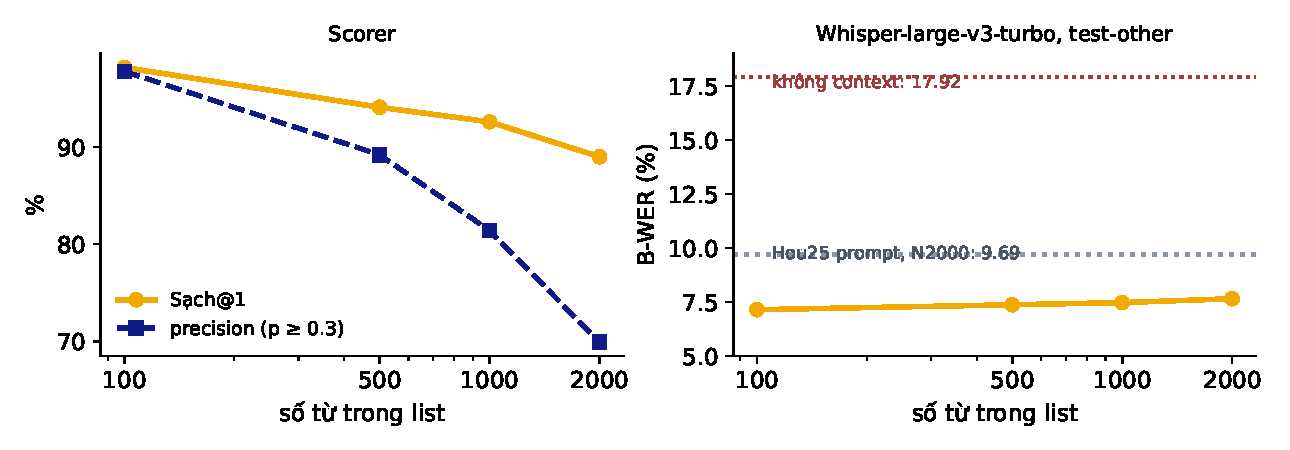
\includegraphics[width=\linewidth]{imgs/theo_N.pdf}
\vspace{0.05cm}

{\footnotesize WER 2.96 / 3.04 / 3.08 / 3.22 (N100 / 500 / 1000 / 2000). Scorer hai nhánh 1 model, $p \geq 0.3$, đẩy có vị trí. Chưa có Hou25 ở N100--1000 trong cùng pipeline.}
\end{columns}
\src{REPORT-1115 mục 3, 6, 6c, 7c}
\end{frame}

\begin{frame}{Dự phòng 3: chi tiết decode và chọn tham số}
\begin{itemize}\footnotesize
\item \textbf{Biết decoder đang nghe giây nào:} cộng attention các alignment head của Whisper, lọc trung vị 7, lấy argmax (Simul-Whisper, arXiv 2406.10052 §2.1).
\item \textbf{Đẩy:} cộng $\lambda$ vào log-prob token của từ khi giây đó nằm trong đoạn của từ $\pm$ 0.05 s; mỗi từ chỉ đẩy token đầu một lần (trước khi chặn: một câu viết ``gordon'' 106 lần).
\item \textbf{Chọn từ:} $p \geq 0.3$ sau khi tranh nhau tại chỗ ($\sim$2.3 từ/câu). $\lambda$ = 5 (không prompt), 3 (có prompt).
\item \textbf{Chọn tham số trên dev-other 400 câu}, không chọn trên test.
\item \textbf{Chống lặp:} greedy Whisper lặp chữ ở vài câu khi bị đẩy hoặc prompt quá ngắn \ra{} decode lại không context khi tỉ lệ nén $>$ 2.4 (như openai-whisper), áp cho \textbf{mọi hệ}.
\item \textbf{Biên mở sớm} làm mất từ thường đứng trước (``the''); biên của nhánh đúng thứ tự gần như không mở sớm (lệch đầu [+0.03; +0.10] s).
\end{itemize}
\end{frame}

\begin{frame}{Dự phòng 4: liên quan và điểm mới (đã tra, chưa đủ để khẳng định ``chưa ai làm'')}
\renewcommand{\arraystretch}{1.18}\scriptsize
\begin{tabular}{L{3.5cm}L{3.5cm}L{6.4cm}}
\toprule
Công trình & Dùng vị trí? & Khác với nhóm \\
\midrule
CB-Whisper (2309.09552) & bản đồ TTS $\times$ audio + CNN & chỉ đưa \textbf{chữ} vào prompt; Hou25 dựa trên ý này \\
CTC-WS (2406.07096), Spike-triggered (2310.04657) & có, theo frame & chỉ cho ASR \textbf{CTC / transducer}; không dùng cho decoder tự hồi quy \\
PTC-Bias (2609.28727) & có khoảng [a, b] & dùng để lọc list và \textbf{sửa sau} khi decode xong \\
Liu et al. (2508.17796) & không & boost cây tiền tố trên Whisper, \textbf{không gate} theo thời gian \\
IBM (2604.12398) & nhãn trên chữ, loss phụ & bỏ đi lúc inference; fine-tune ASR \\
\midrule
\textbf{Nhóm} & \textbf{có, từ scorer} & đẩy logit \textbf{đúng lúc} cho decoder tự hồi quy \textbf{đóng băng}, không prompt; scorer hai nhánh ra vị trí \\
\bottomrule
\end{tabular}
\vspace{0.15cm}

{\footnotesize Nguồn: \texttt{related-work/novelty-gate.md}. Một số mục mới đọc tóm tắt; cần đọc toàn văn trước khi viết bài.}
\end{frame}

\end{document}
